\documentclass[12pt]{article}
\usepackage[margin=0.5in]{geometry}
\usepackage{graphicx}
\usepackage{xcolor}
\usepackage{amsmath}
\usepackage{amsfonts}
\usepackage{amssymb}
\usepackage{cleveref}

\newcommand{\hl}[1]{\colorbox{yellow}{#1}}

\newcommand{\vA}{\mathbf{A}}
\newcommand{\vB}{\mathbf{B}}
\newcommand{\vC}{\mathbf{C}}
\newcommand{\vu}{\mathbf{u}}
\newcommand{\bw}{\mathbf{w}}
\newcommand{\vw}{\mathbf{w}}
\newcommand{\bv}{\mathbf{v}}
\newcommand{\vv}{\mathbf{v}}
\newcommand{\vf}{\mathbf{f}}
\newcommand{\vr}{\mathbf{r}}
\newcommand{\cQnet}{\mathcal{Q}_{\text{net}}}
\newcommand{\cP}{\mathcal{P}}
\newcommand{\bk}{\mathbf{k}}
\newcommand{\cQ}{\mathcal{Q}}
\newcommand{\vPhi}{\boldsymbol{\Phi}}
\newcommand{\bu}{\mathbf{u}}
\newcommand{\bepsilon}{\boldsymbol{\epsilon}}
\newcommand{\bsigma}{\boldsymbol{\sigma}}
\newcommand{\phii}{\phi^{(i)}}
\newcommand{\phij}{\phi^{(j)}}
\newcommand{\Ti}{T^{(i)}}
\newcommand{\Tj}{T^{(j)}}
\newcommand{\ui}{u^{(i)}}
\newcommand{\uj}{u^{(j)}}
\newcommand{\vui}{\mathbf{u}^{(i)}}
\newcommand{\vuj}{\mathbf{u}^{(j)}}
\newcommand{\Ei}{E^{(i)}}

% d#/dt
\newcommand{\ddt}[1]{\frac{\dd #1}{\dd t}}
\newcommand{\ddtb}[1]{\frac{\dd^2#1}{\dd t^2}}
\newcommand{\ddtn}[2]{\frac{\dd^#2#1}{\dd t^#2}}
% p#/pt
\newcommand{\ppt}[1]{\frac{\partial#1}{\partial t}}
\newcommand{\pptb}[1]{\frac{\partial^2#1}{\partial t^2}}
\newcommand{\pptn}[2]{\frac{\partial^#2#1}{\partial t^#2}}

\newcommand\vn{{\mathbf{n}}}

\begin{document}

\begin{abstract}
    This work presents a physics-infused reduced-order modeling (PIROM) framework towards the design, analysis, and optimization of ablating hypersonic thermal protection systems (TPS). 
\end{abstract}

\section{Introduction}


\section{Modeling of Ablating Thermal Protection Systems}

This section presents the ablation problem for a non-decomposing TPS as a parametrized system of non-linear PDEs. These non-linear PDEs govern the energy of heat conduction and the pseudo-elastic material deformation of the mesh motion. Two different but mathematically-connected numerical solution strategies are provided: (1) a high-fidelity full-order model (FOM) based on a discontinuous Galerkin FEM, and (2) a thermo-elastic RPM based on a one-dimensional approximation to the energy and pseudo-elasticity equations.

\subsection{Governing Equations}\label{sec_governing_equations}

Consider a generic domain $\Omega\subset$, $d=2$ or $3$, illustrated in Fig.~\ref{fig_general_domain}. A heat flux $q_b(x,t)$ is prescribed on the boundary $\Gamma_q$ (i.e., Neumann boundary condition), and the temperature $T_b(x,t)$ is prescribed on boundary $\Gamma_T$ (i.e., Dirichlet boundary condition), where $\Gamma_q\cup\Gamma_T = \partial\Omega$ and $\Gamma_q\cap\Gamma_T = \emptyset$. The ablation occurs only on the heated boundary $\Gamma_q$, and its effects are included into the energy equation using an Arbitrary Lagrangian-Eulerian (ALE) description. The ALE assumes that the displacement $\vw(x,t)\in\mathbb{R}^d$ of the computational mesh moves with velocity $\vv(x,t)$ that is different to the material velocity, which is fixed to zero in this work.

\begin{figure}
    \centering
    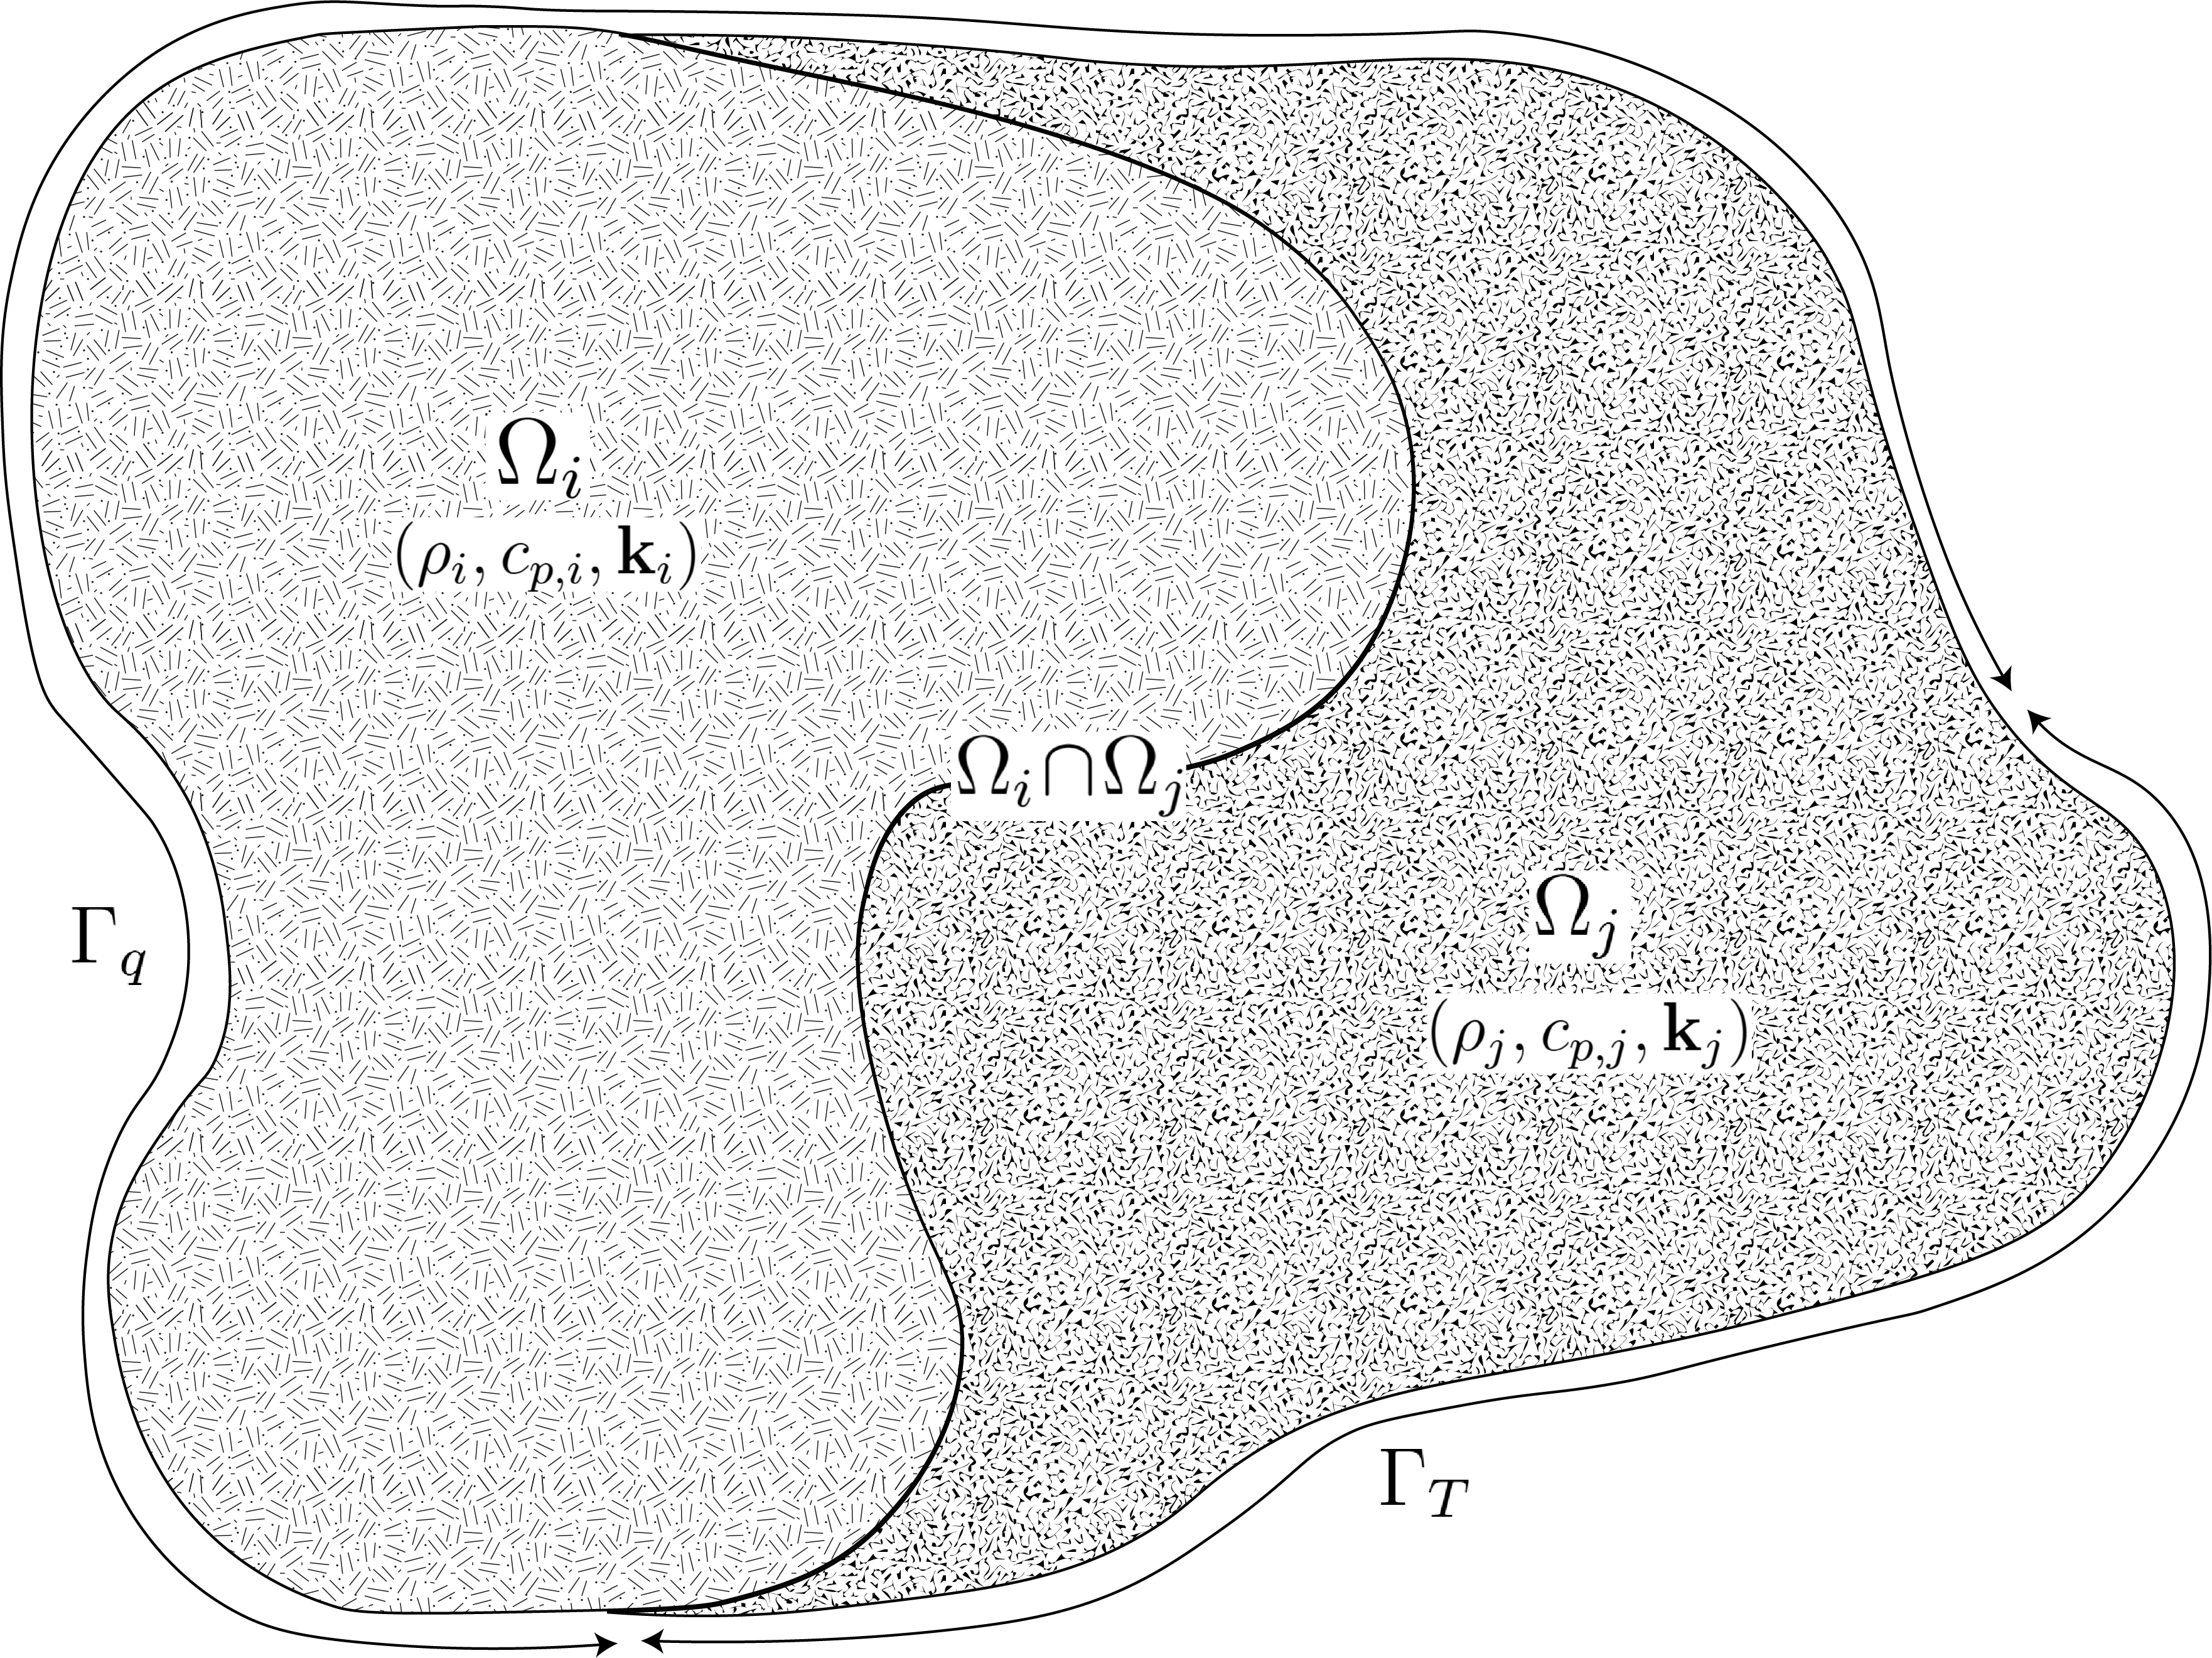
\includegraphics[width=0.6\textwidth]{./figs/general_domain.png}
    \caption{General domain $\Omega$ with prescribed heat flux $q_b(x,t)$ and temperature $T_b(x,t)$ on the boundaries $\Gamma_q$ and $\Gamma_T$, respectively. The mesh moves with a velocity $\mathbf{v}(x,t)$, while the material velocity is $\mathbf{w}(x,t)$.\hl{draw mesh next to arbitrary domain with moving boundaries.}}
    \label{fig_general_domain}
\end{figure}

The transient heat conduction is described by the energy equation,
\begin{subequations}
    \begin{align}
        \rho c_p\left(\ppt{T} - \mathbf{v}(x,t)\cdot\nabla T\right) - \nabla\cdot (\mathbf{k}\nabla T) &= \cQ(x,t),\ x\in\Omega \label{eqn_thermal_pde}\\
        -\mathbf{k}\nabla T\cdot \vn &= q_b(x,t),\ x\in\Gamma_q\label{eqn_thermal_bc_neumann}\\
        T(x,t) &= T_b(x,t),\ x\in\Gamma_T\label{eqn_thermal_bc_dirichlet}\\
        T(x,0) &= T_0(x),\ x\in\Omega\label{eqn_thermal_ic}
    \end{align}\label{eqn_governing_equations}
\end{subequations}
while the mesh motion is described by the pseudo-elasticity equation,
\begin{subequations}
    \begin{align}
        \nabla\cdot\boldsymbol{\sigma}(\mathbf{w}) &= 0\label{eqn_elasticity_pde}\\
        \vw(x,t) &= \vw_q(x,t),\quad x\in\Gamma_q\label{eqn_displacement_heated_bc}\\
        \vw(x,t) &= 0,\quad x\notin \Gamma_q\label{eqn_displacement_unheated_bc}\\
        \vw(x,0) &= \boldsymbol{0}\label{eqn_displacement_initial_condition}
    \end{align}
\end{subequations}

The density $\rho$, heat capacity $c_p$, and thermal conductivity $\mathbf{k}\in\mathbb{R}^{n_d\times n_d}$ are assumed to be constant with respect to temperature in this work. The terms in \cref{eqn_thermal_pde}, in the order they appear, correspond to the unsteady energy storage, heat conduction, temperature advection due to mesh motion, and the heat source terms. 

The elasticity equation \cref{eqn_elasticity_pde} states that the divergence of the stress tensor $\boldsymbol{\sigma}(\mathbf{w})$ is zero. The stress tensor is related to the strain tensor $\bepsilon(\bw)$ through Hooke's law,
\[
    \boldsymbol{\sigma}(\bw) = \mathbb{D}:\boldsymbol{\epsilon}(\bw)
\]
where $\mathbb{D}$ is the constitutive operator, ``:'' is the double contraction of tensors, and $\bepsilon$ is the symmetric strain tensor given by,
\[
    \bepsilon(\bw) = \frac{1}{2}\left(\nabla\bw + \nabla\bw^T\right)
\]
For instance, an isotropic material assumption results in,
\[
    \bsigma = \lambda\left(\nabla\cdot\bw\right) \mathbf{I} + 2\mu\bepsilon(\bw)
\]
where $\lambda$ and $\mu$ are Lame constants that are arbitrarily selected to model the mesh motion. The ``material'' properties $\lambda$ and $\mu$ can be chosen to tailor the mesh deformation and need not represent the actual material being modeled~\hl{Amar2016}. 

The boundary conditions for the energy equation includes a heated surface (\cref{eqn_thermal_bc_neumann}) and a constant-temperature surface (\cref{eqn_thermal_bc_dirichlet}). The boundary conditions for the pseudo-elasticity equation are a function of the surface temperature $T_q(x,t)$ for $x\in\Gamma_q$ using a B' table. The B' table....
\begin{equation}
    \bw_q(x,t) = \int_{0}^{t} \mathbf{v}(x,\tau)d\tau = \int_{0}^{t}\mathbf{f}\left(T_q(x,\tau)\right)d\tau\label{eqn_boundary_displacement}
\end{equation}


\subsection{Full-Order Model: Finite-Element Method}\label{sec_fom}

To obtain the full-order numerical solution, the governing equation is spatially discretized using the variational principle from Discontinuous Galerking (DG) to result in a high-dimensional system of ODEs for the time-varying nodal data. The full-order TPS ablation simulations are computed using standard FEM instead, and the equivalence between DG and standard FEM is noted upon their convergence.

Consider a conforming mesh partition domain, where each element belongs to one and only one component. Denote the collection of all $M$ elements as $\left\{E_i\right\}_{i=1}^{M}$. In an element $E_i$, its shared boundaries with another element $E_j$, Neumann BC, and Dirichlet BC are denoted as $e_{ij}$, $e_{iq}$, and $e_{iT}$, respectively. Lastly, $\left|e\right|$ denotes the length $(n_d=2)$ or area $(n_d=3)$ of a component boundary $e$.

For the $i$-th element, use a set of $n^{(i)}$ trial functions, such as polynomials, to represent the temperature distribution,
\begin{equation}
    T^{(i)}(x,t) = \sum_{i=1}^{n^{(i)}} \phi_i^{(i)}(x)u_i^{(i)} \equiv \boldsymbol{\phi}^{(i)}(x)^T\vu^{(i)}(t)\label{eqn_element_temperature}
\end{equation}


By standard variational processes, e.g., \hl{Cohen2018}, the full governing equation is denoted as,
\begin{equation}
    \vA(\vu)\dot{\vu} = \left(\vB(\vu) + \vC(t)\right)\vu + \mathbf{f}(t)\label{eqn_energy_fem}
\end{equation}
where $\vu = \left(\vu^{(1)}, \vu^{(2)}, \ldots, \vu^{(M)}\right)^T\in\mathbb{R}^{MP}$ includes all the DG variables, $\mathbf{f}\in\mathbb{R}^{MP}$ is the external forcing, and the system matrices $\vA$, $\vB$, and $\vC$ are due to heat capacity, heat conduction, and temperature advection, respectively. The detailed formulation of the DG model is provided in Appendix~\hl{DG-FEM}.

\subsection{Reduced-Physics Model: Lumped-Capacitance Model}

This section presents the main results regarding the derivation of the LCM for ablating materials, and the main details are provided in Appendix~\hl{x}. The RPM is based on a coarse-grained temperature approximation in each component, neglecting higher-order spatial information that is critical to predict surface temperatures and thus the rate of surface recession. 

\subsubsection{Finite-Element Method and Component Interactions}

The arbitrary domain in Fig.~\ref{fig_general_domain} is partitioned into $N$ components $\left\{\Omega^{(i)}\right\}_{i=1}^{N}$, each with $\left\{E^{(i)}_j\right\}_{j=1}^{n^{(i)}}$ finite elements, establishing the resolution for the temperature and mesh displacement fields over each component. Figure~\hl{x} shows a partition of the TPS into $N=M=3$, where the top and bottom are subject to Neumann and adiabatic boundary conditions, respectively. 

\begin{figure}
    \centering
    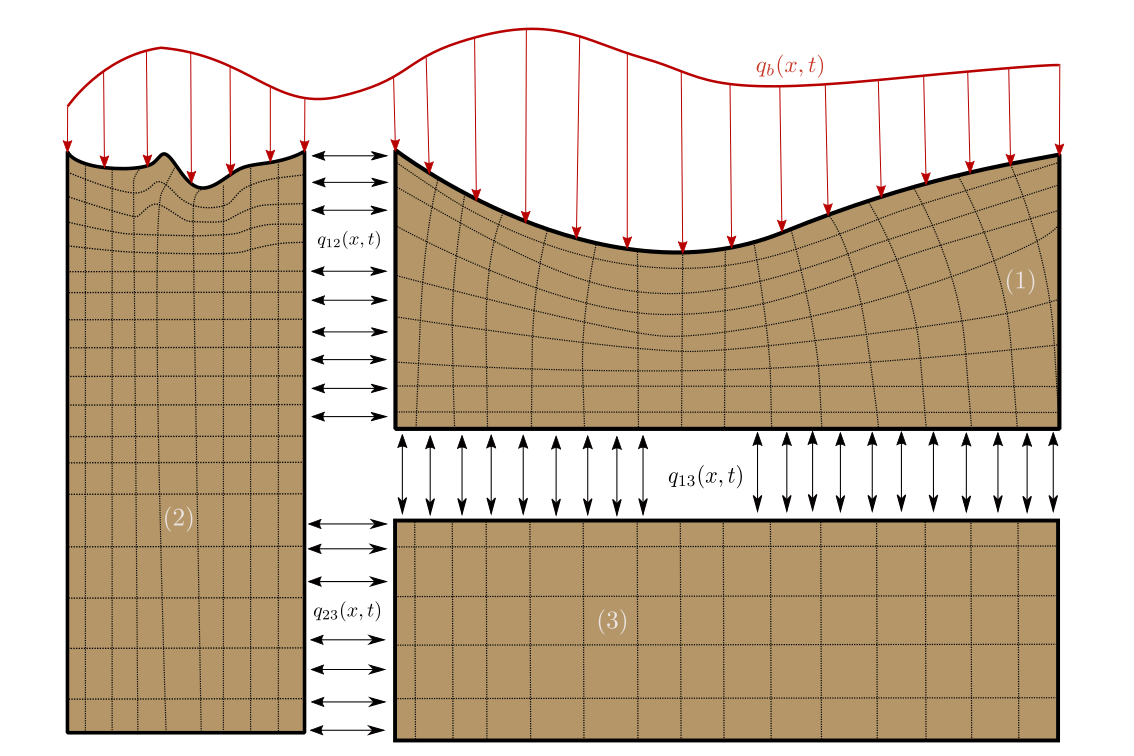
\includegraphics[width=0.8\textwidth]{./figs/three_components.png}
    \caption{Partition of the TPS into three one-dimensional components.}
    \label{fig_domain_partition}
\end{figure}

A first-order FEM scheme is adopted for each component, which results in a block-diagonal system of ODEs for the nodal temperature values of the components,
\begin{equation}
    \vA\left(\bvu\right)\dot{\bvu} = \left(\vB + \vC(t)\right)\bvu + \vf\left(\bvu,t\right)\label{eqn_rpm}
\end{equation}
where the block matrices are defined as,
\begin{subequations}
\begin{align}
\begin{aligned}
    \vA_{ij} &= \begin{cases}
        \vA^{(i)}(\bvu^{(i)}), & i=j \\
        0, & i\neq j
    \end{cases}\\
    \vB_{ij} &= \begin{cases}
        \vB^{(i)}(\bvu^{(i)}), & i=j \\
        0, & i\neq j
    \end{cases}
\end{aligned}
&\qquad
\begin{aligned}
    \vC_{ij}(t) &= \begin{cases}
        \vC^{(i)}(t), & i=j \\
        0, & i\neq j
    \end{cases}\\
    \mathbf{f}_i(\bvu,t) &= \begin{cases}
        \mathbf{f}^{(i)}_{\text{BC}}(t)+\mathbf{f}^{(i)}_{\cQ}(\bvu,t), & i=j \\
        \boldsymbol{0}, & i\neq j
    \end{cases}
\end{aligned}\label{eqn_rpm_matrices}
\end{align}
\end{subequations}
where $\vfBC$ and $\vfQ$ are the boundary and component-level energy sources. 


\subsubsection{Coarse Graining}

Consider a DG model as in ~\cref{eqn_energy_fem} for $M$ components and $N$ elements; clearly $N\gg N$. Let $\cV_j=\left\{i | E^{(i)}\in\Omega^{(j)}\right\}$ be the indices of the elements belonging to the $j$-th component, so $E^{(i)}\in\Omega^{(j)}$ for $i\in\cV_j$; number of elements in $\Omega^{(j)}$ is denoted as $\left|\cV_j\right|$.



The ablation on the $i$-th component is modeled using a one-dimensional approximation to the temperature and mesh-motion equations in \cref{eqn_governing_equations}, and are given by,
\begin{subequations}
    \begin{align}
        \rho c_p\left(\frac{\partial T^{(i)}}{\partial t} - v^{(i)}(x,t)\frac{\partial T^{(i)}}{\partial x}\right) - \frac{\partial}{\partial x}\left(k\frac{\partial T^{(i)}}{\partial x}\right) - \cQ^{(i)}_{\text{net}}(x,t) &= 0\label{eqn_thermal_1d}\\
        \frac{\partial}{\partial x}\left(\frac{\partial u^{(i)}}{\partial x}\right) &= 0\label{eqn_elasticity_1d}
    \end{align}\label{eqn_rpm}
\end{subequations}
with boundary conditions for the energy equation,
\begin{subequations}
    \begin{align}
        -k\frac{\partial T^{(i)}}{\partial x}\Bigg|_{x=0} &= q^{(i)}_b(t)\\
        -k\frac{\partial T^{(i)}}{\partial x}\Bigg|_{x=\ell} &= 0
    \end{align}
\end{subequations}
and for the elasticity equation,
\begin{subequations}
    \begin{align}
        u^{(i)}(0,t) &= \int_{t_0}^{t}v^{(i)}(\tau)d\tau = \int_{0}^{t} f(T^{(i)}_w(\tau))d\tau\\
        u^{(i)}(\ell,t) &= 0
    \end{align}
\end{subequations}
where $v^{(i)}(t)$ is the surface receding velocity due to ablation, which is a function of the surface temperature as in \cref{eqn_boundary_displacement}. The surface velocity is computed from a cubic spline interpolate to a B' look-up table...



\subsubsection{Thermal Solver}

The FEM implementation details are supplied in Appendix~\hl{x}. For the $n$-th component, the result of the FEM discretization is a system of ODEs for the nodal temperatures, coupled to the neighboring component $n+1$ through the energy volumetric source term,
\begin{equation}
    \mathbf{A}^{(i)}\frac{d\mathbf{T}^{(i)}}{dt} + \left(\mathbf{B}^{(i)} - \mathbf{C}^{(i)}(t)\right)\mathbf{T}^{(i)} = \mathbf{f}^{(i)}(t)
\end{equation}
where,
\begin{itemize}
    \item $\mathbf{A}^{(i)}\in\mathbb{R}^{M\times M}$ is the mass matrix,
    \item $\mathbf{B}^{(i)}\in\mathbb{R}^{M\times M}$ is the stiffness matrix,
    \item $\mathbf{C}^{(i)}(t)\in\mathbb{R}^{M\times M}$ is the advection matrix,,
    \item $\mathbf{T}^{(i)}\in\mathbb{R}^{M}$ is the vector of nodal temperatures, and
    \item $\mathbf{f}^{(i)}(t)\in\mathbb{R}^{M}$ is the input vector, which includes the Neumann boundary conditions and the net volumetric energy source term $\cQ^{(i)}_{\text{net}}$.
\end{itemize}
where $M$ is the number of nodes in the one-dimensional mesh for the $i$-th component.

\subsubsection{Pseudo-Elastic Solver}

Note that \cref{eqn_elasticity_1d} is steady. Under the assumption that the mesh deformation is quasi-steady, it can be applied at each time step within an ablation simulation. For instance, a known value of the wall temperature $T_w(t)$ specifies a Dirichlet boundary condition for the displacement, and the resulting nodal displacements within the ablator are determined from \cref{eqn_elasticity_pde}.

Along the one-dimensional domain, the PDE in \cref{eqn_elasticity_pde} simplifies to,
\begin{equation}
    \frac{\partial^2 u^{(i)}}{\partial x^2} = 0
\end{equation}
which has the analytical solution,
\begin{equation}
    u^{(i)}(x,t) = a(t)x + b(t)
\end{equation}
Imposing the boundary conditions leads to,
\begin{equation}
    u^{(i)}(x,t) = u^{(i)}(0,t)\left(\frac{x_1^{(i)} - x}{h^{(i)}}\right)
\end{equation}
The mesh velocity is the time derivative of the displacement,
\begin{equation}
    v^{(i)}(x,t) = \frac{\partial u^{(i)}(x,t)}{\partial t} = v^{(i)}(t)\left(\frac{x_1^{(i)} - x}{h^{(i)}}\right)
\end{equation}

\subsubsection{Coupling Scheme}

\subsubsection{Reduced-Physics Ablation Simulation}








\section{Physics-Infused Reduced-Order Modeling}\label{sec_pirom}
The formulation of PIROM for ablating TPS starts by connecting the FOM, i.e., DG-FEM, and the RPM, i.e., the LCM, via a coarse-graining procedure. This procedure pinpoints the missing dynamics in the LCM when compared to DG-FEM. Subsequently, the Mori-Zwanzig (MZ) formalism is employed to determine the model form for the missing dynamics in PIROM. Lastly, the data-driven identification of the missing dynanmics in PIROM is presented.

\subsection{Deriving the Reduced-Physics Model via Coarse-Graining}
The LCM is derived from a full-order DG on a fine mesh via a projection process, i.e., coarse graining. This process constraints the trial function space of a full-order DF model to a subset of piece-wise constants, so that the variables $\vu$, matrices $\vA$, $\vB$, and $\vC$, and forcing vector $\vf$ are all approximated using a single state associated to the average temperature. The details of the projection are described next.

\subsubsection{Coarse-Graining of States}

Consider a DG model as in \cref{eqn_full_dg} for M elements and an LCM as in \cref{eqn_lcm} for $N$ components; clearly $M\gg N$. 


\appendix

\section{Numerical Implementation}\label{app_implementation}

\subsection{Full-Order Model}

\subsection{Reduced-Physics Model}

This section outlines the DG-FEM implementation for the RPM with $N=3$ inter-connected one-dimensional components used in Sec.~\hl{x}. Consider the splitting of the TPS as in Fig.~\hl{x}. Over the $i$-th element with $x\in\Omega^{(i)}(t)$, consider the following linear basis set $\phi_k^{(i)}(x)$ with $k=1,2$ on the element $[x^{(i)}_{0}(t),x^{(i)}_{1}(t)]$ with length $h^{(i)}(t)=x^{(i)}_{1}(t) - x^{(i)}_{0}(t)$. For notational convenience, the time dependence of the spatial domain due to ablating surfaces is dropped. The orthogonal basis functions are defined as,
\begin{equation}
    \phi^{(i)}_1(x) = 1,\quad \phi^{(i)}_2(x) = \frac{2}{h^{(i)}}\left(x - x^{(i)}_c\right)
\end{equation}
where $x^{(i)}_c = (x^{(i)}_0 + x^{(i)}_1) / 2$. Let,
\[
    x(\xi) = \frac{1-\xi}{2}x^{(i)}_0 + \frac{1 + \xi}{2}x^{(i)}_{1}
\]
thus for $\xi\in[-1,1]$,
\begin{equation}
    \hat{\phi}^{(i)}_1(\xi) = 1, \quad \hat{\phi}^{(i)}_2(\xi) = \xi
\end{equation}

Multiply through by the weight function $\phi_j(x)$ and integrate over the domain $\Omega^{(i)}$,
\begin{equation}
    \int_{\Omega}\left[\rho c_p\left(\frac{\partial T^{(i)}}{\partial t} - v^{(i)}(x,t)\frac{\partial T^{(i)}}{\partial x}\right) - \frac{\partial}{\partial x}\left(k\frac{\partial T^{(i)}}{\partial x}\right) - \cQ^{(i)}_{\text{net}}(x,t)\right]\phii_l(x)dx = 0
\end{equation}
Using integration by parts the natural boundary conditions are obtained,
\begin{align}
    \int_{\Omega}\rho c_p\left(\frac{\partial\Ti}{\partial t}\phii_l(x) - v(x,t)\frac{\partial\Ti}{\partial x}\phii_l(x)\right)dx &+ \int_{\Omega} k\frac{\partial\Ti}{\partial x}\frac{\partial\phii_l(x)}{\partial x} dx\notag\\
    &=k\frac{\partial\Ti}{\partial x}\phii_l(x)\Bigg|_{\partial\Omega} + \int_{\Omega}\phii_l(x)\cQ(x,t)dx
\end{align}
Perform the finite-element approximation,
\begin{equation}
    T^{(i)}(x,t)\approx\sum_{k=1}^{n^{(i)}}\ui_k(t)\phii_k(x)
\end{equation}
and define the matrix elements,
\begin{align}
    A^{(i)}_{kl} &= \int_{\Omega}\rho c_p\phii_k(x)\phii_l(x)dx\\
    B^{(i)}_{kl} &= \int_{\Omega}k\frac{\partial\phii_k(x)}{\partial x}\frac{\partial\phii_l(x)}{\partial x}dx\\
    C^{(i)}_{kl}(t) &= \int_{\Omega}\rho c_p v^{(i)}(x,t)\phii_k(x)\frac{\partial\phii_l}{\partial x}dx\\
    f^{(i)}_l(t) &= k\frac{\partial T}{\partial x}\phii_l(x)\Bigg|_{\partial\Omega} + \int_{\Omega}\phii_l(x)\cQnet^{(i)}(x,t)dx
\end{align}
The time-dependent finite-dimensional ODE system for nodal temperatures $\mathbf{T}(t)$, including the ALE-induced advection effect from mesh motion, is given as,
\begin{equation}
    \mathbf{A}\frac{d\mathbf{T}}{dt} + \left(\mathbf{B} - \mathbf{C}(t)\right)\mathbf{T} = \mathbf{f}(t)
\end{equation}

On the element $(e)$ the expressions for mass, stiffness, advection, and forcing are given as,
\begin{align}
    M^{(i)}_{mn} &= \int_{x^{(i)}_i}^{x^{(i)}_{i+1}}\rho c_p\phi^{(i)}_m(x)\phi^{(i)}_n(x)dx = \rho c_p \frac{h^{(i)}}{6}\begin{pmatrix}
        2 & 1 \\ 1 & 2
    \end{pmatrix}\\
    K^{(i)}_{mn} &= \int_{x^{(i)}_i}^{x^{(i)}_{i+1}} k^{(i)} \frac{\partial \phi^{(i)}_m}{\partial x}\frac{\partial \phi^{(i)}_n}{\partial x} dx = \frac{k}{h_e}\begin{pmatrix}
        1 & -1 \\ -1 & 1
    \end{pmatrix}\\
    C^{(i)}_{mn}(t) &= \int_{x_i}^{x_{i+1}}\rho c_p v(x,t) \frac{\partial \phi_n(x)}{\partial x}\phi_m(x) dx\\
    f^{(i)}_1(t) &= \left(q(t),0\right)^T
\end{align}



The thermodynamic interaction between the components is modeled via the net volumetric energy source from \cref{eqn_net_volumetric_energy}, which for the three-components in Fig.~\hl{x} are described by,
\begin{subequations}
    \begin{align}
        \cQ^{(1)}_{\text{net}}(x,t) &= -\cQ^{(1,2)}(x,t)\\
        \cQ^{(2)}_{\text{net}}(x,t) &= \cQ^{(1,2)}(x,t) - \cQ^{(2,3)}(x,t)\\
        \cQ^{(3)}_{\text{net}}(x,t) &= \cQ^{(2,3)}(x,t)
    \end{align}
\end{subequations}




\end{document}
